\documentclass[14pt]{article}

\usepackage[letterpaper,bindingoffset=0.2in,%
            left=1in,right=1in,top=1in,bottom=1in,%
            footskip=.25in]{geometry}
\usepackage[english]{babel}
\usepackage[section]{placeins}
\usepackage{float}
\usepackage[utf8x]{inputenc}
\usepackage{amsmath}
\usepackage{amssymb}
\usepackage{amsthm}
\usepackage{MnSymbol}
\usepackage{graphicx}
\usepackage[makeroom]{cancel}
\usepackage{booktabs}
\usepackage{enumitem}
\usepackage{tabularx}
\usepackage{xcolor}
\usepackage{hyperref}
\usepackage{tikz}
\usepackage{pgfplots}
\pgfplotsset{compat=1.11}
\usepackage{systeme}
\usepackage{calc}
\usepackage{caption}
\usepackage{subcaption}
\usepackage{multicol}
\usepackage{listings}

\lstset{language=Python}

\usetikzlibrary{calc}
\usetikzlibrary{positioning}
\usetikzlibrary{arrows,decorations.markings}

\graphicspath{ {./images/} }


% DOCUMENT STARTS HERE

\begin{document}

\title{Analysis H Project: \\ \textbf{3D Graphics Generation with Matrices}}
\author{Mihir Rao}
\maketitle

\begin{center}
	\vspace{3em}
	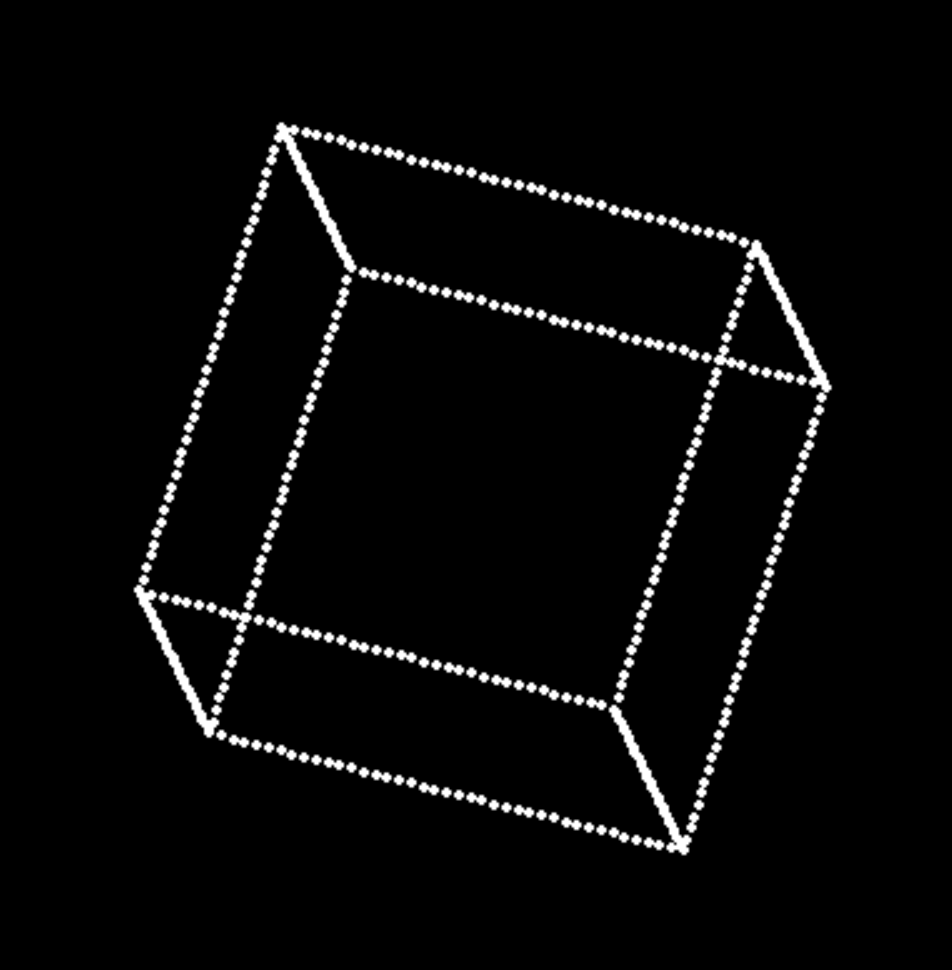
\includegraphics[scale=0.8]{titleImg}
	\vspace{3em}
\end{center}

\section*{Overview}

For our Analysis H project, Steve and I decided to dive into the realm of computer graphics and matrices' applications in this field. Specifically, we wrote code that generates 3D points, projects these 3D points onto a 2D surface(the computer screen), and transforms these points to display an animation(using matrices). We both were fascinated by the numerous applications of matrices and thought this will be a fun project to work on. After doing further research, it also turns out that Renderman, Pixar's animation software, is heavily based on matrices and linear algebra; so this was the perfect time for us to dip our toes in the fundamentals of this field. This document serves to explain how we came up with the math of this code, challenges we faced, and the ultimate solutions to those challenges. The next section is a brief introduction of how we approached the code and following that is the actual math behind it. Enjoy!

\newpage

\section*{The Math}

There are many aspects of the code that we had to come up with in order to display an animated 3D object on a 2D screen. Some of these aspects rely more on math than others and this document will go over those functions in \textcolor{blue}{\href{https://github.com/itsmehere/SpinningCube/blob/main/cubeProj.py}{this code}}.

\subsection*{Coordinate Setup \& Matrices}

\begin{figure}[!htb]
    \centering
    \subfloat[\centering]{{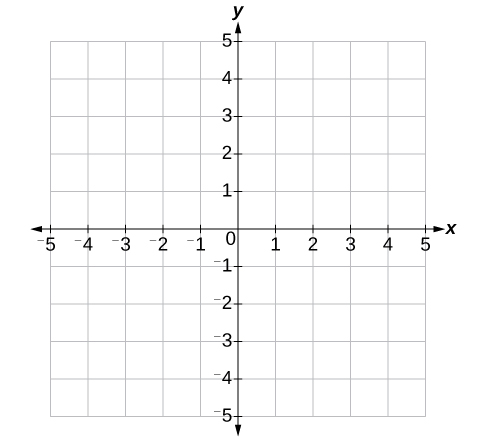
\includegraphics[width=5cm]{cartesianCoordinates} }}%
    \qquad
    \subfloat[\centering]{{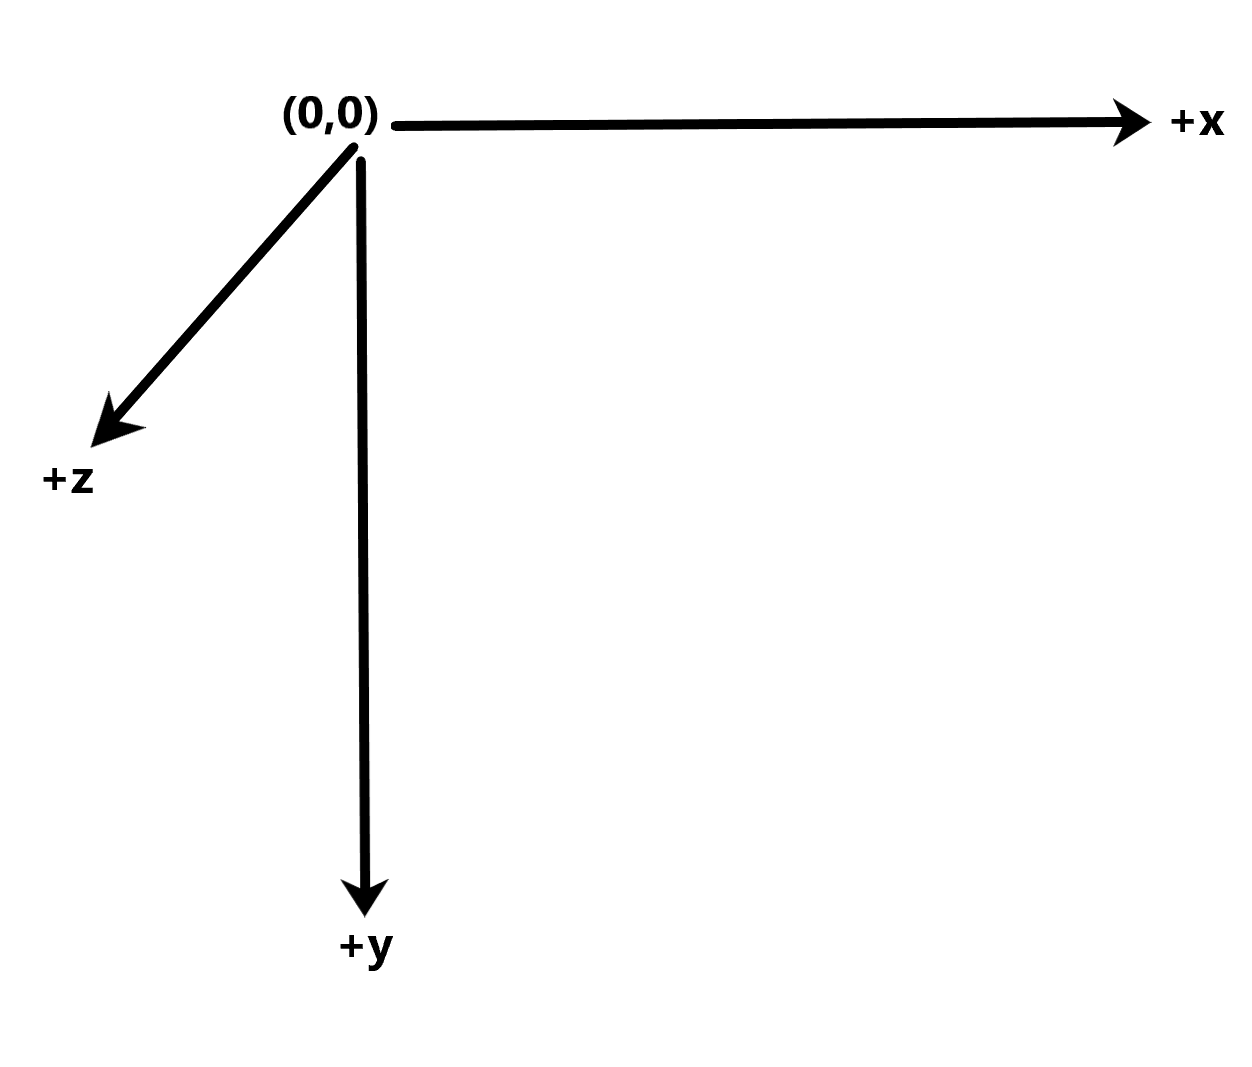
\includegraphics[width=5cm]{computerCoordinates} }}%
    \caption{Coordinates}%
    \label{fig:example}%
\end{figure}

In the figures above, we see (a): our regular cartesian coordinate system where (0,0) is at the center of the screen and we have 4 quadrants. However, in figure (b), we see a generic computer coordinate system--where (only the 4th quadrant is included making the origin the top left of the screen. Though it may seem more complex to display animations at a point other than the origin, computer screen layouts actually make this problem easier(with a little bit more math of course) since we no longer have to deal with negative values. So why is this important? Well, if we wanted to display an object at the center of the screen, or in fact, any point other than the origin, we'd have to come up with some sort of way to cleverly use matrices and transformations. We'll start of with our generic 2 x 2 rotation matrix.

\vspace{1em}

\begin{figure}[h]
	\vspace*{1em}
	\begin{center}
		\begin{minipage}[b]{0.45\textwidth}
			\centering
			
			$$
			\begin{bmatrix}
			cos(\theta) & -sin(\theta) \\
			sin(\theta) & cos(\theta)
			\end{bmatrix}
			$$
		\end{minipage}
		\hfill
		\begin{minipage}[b]{0.45\textwidth}
			\centering
			$$
			\begin{bmatrix}
			1 & 0 \\
			0 & 1
			\end{bmatrix}			
			$$
		\end{minipage}
	\end{center}
	\vspace*{1em}
\end{figure}

\vspace{1em}

A couple things that are important to note before we proceed are that this matrix rotates points in 2 dimensions and on the $xy$ plane--meaning around the $z$ axis. Since we need to go into 3D, we need to change this matrix to work for 3D points and we can do that by using the concept of an identity matrix. Shown as the top right matrix, we can multiply the rotation matrix by this and still obtain the same rotation matrix. A 3x3 identity matrix is the just the same and we can use that concept to come up with a rotation matrix for 3D. These new matrices are shown below.

\begin{figure}[h]
	\vspace*{1em}
	\begin{center}
		\begin{minipage}[b]{0.45\textwidth}
			\centering
			
			$$
			\begin{bmatrix}
			cos(\theta) & -sin(\theta) & 0 \\
			sin(\theta) & cos(\theta) & 0 \\ 
			0 & 0 & 1
			\end{bmatrix}
			$$
		\end{minipage}
		\hfill
		\begin{minipage}[b]{0.45\textwidth}
			\centering
			$$
			\begin{bmatrix}
			1 & 0 & 0 \\
			0 & 1 & 0 \\
			0 & 0 & 1
			\end{bmatrix}			
			$$
		\end{minipage}
	\end{center}
	\vspace*{1em}
\end{figure}

Just like we can add on another row and column to the identity matrix, to get the matrix for the new dimension, we can do the same for the rotation matrix. To prove this works, we can take any point and verify its coordinates using both matrices.

\vspace*{1em}

\begin{equation}
	\begin{bmatrix}
	cos(\theta) & -sin(\theta) & 0 \\
	sin(\theta) & cos(\theta) & 0 \\ 
	0 & 0 & 1
	\end{bmatrix}
	\begin{bmatrix}
	1 \\
	0 \\ 
	0
	\end{bmatrix}	
	=
	\begin{bmatrix}
	cos(\theta) \\
	sin(\theta) \\ 
	0
	\end{bmatrix}
\end{equation}

\vspace*{1em}

\begin{equation}
	\begin{bmatrix}
	cos(\frac{\pi}{2}) & -sin(\frac{\pi}{2}) & 0 \\
	sin(\frac{\pi}{2}) & cos(\frac{\pi}{2}) & 0 \\ 
	0 & 0 & 1
	\end{bmatrix}
	\begin{bmatrix}
	1 \\
	0 \\ 
	0
	\end{bmatrix}	
	=
	\begin{bmatrix}
	cos(\frac{\pi}{2}) \\
	sin(\frac{\pi}{2}) \\ 
	0
	\end{bmatrix}
\end{equation}

\vspace*{1em}

\begin{equation}
	\begin{bmatrix}
	0 & -1 & 0 \\
	1 & 0 & 0 \\ 
	0 & 0 & 1
	\end{bmatrix}
	\begin{bmatrix}
	1 \\
	0 \\ 
	0
	\end{bmatrix}	
	=
	\begin{bmatrix}
	0 \\
	1 \\ 
	0
	\end{bmatrix}
\end{equation}

\vspace*{1em}

As we can see above, we get the correct answer of (0, 1, 0) after rotating the point (1, 0, 0) by $\frac{\pi}{2}$ radians counter clockwise. Similarly, we can do this to the rotation matrices of not only the $z$ axis but also the $y$ and $x$ axes. Once we do this, we get the 3 rotation matrices for the $x$, $y$, and $z$ axes.

\begin{figure}[h]
	\vspace*{1em}
	\begin{center}
		\begin{minipage}[b]{0.3\textwidth}
			\centering
			
			$$
			\begin{bmatrix}
			1 & 0 & 0 \\
			0 & cos(\theta) & -sin(\theta) \\ 
			0 & sin(\theta) & cos(\theta)
			\end{bmatrix}
			$$
		\end{minipage}
		\hfill
		\begin{minipage}[b]{0.3\textwidth}
			\centering
			$$
			\begin{bmatrix}
			cos(\theta) & 0 & sin(\theta) \\
			0 & 1 & 0 \\
			-sin(\theta) & 0 & cos(\theta)
			\end{bmatrix}			
			$$
		\end{minipage}
		\hfill
		\begin{minipage}[b]{0.3\textwidth}
			\centering
			$$
			\begin{bmatrix}
			cos(\theta) & -sin(\theta) & 0 \\
			sin(\theta) & cos(\theta) & 0 \\
			0 & 0 & 1
			\end{bmatrix}			
			$$
		\end{minipage}
	\end{center}
	\begin{center}
		\begin{minipage}[t]{0.3\textwidth}
			\caption*{Rotation Matrix $X$}
		\end{minipage}
		\hfill
		\begin{minipage}[t]{0.3\textwidth}
			\caption*{Rotation Matrix $Y$}
		\end{minipage}
		\hfill
		\begin{minipage}[t]{0.3\textwidth}
			\caption*{Rotation Matrix $Z$}
		\end{minipage}
	\end{center}
\end{figure}

(NOTE: Derivations of these 	matrices have been left out to keep paper length minimal). Now that we have our 3 main matrices, we can go back to the problem of a computer's coordinate system. If we were to use just these matrices themselves, our points would be rotating about the origin and the center of the cube would not stay fixed. So how might we solve this problem? One way to solve this problem is using translation matrices. First, we translate the entire cube to the origin, rotate it at the origin, and then translate the entire cube back by using the inverse of the first translation matrix. To create these translation matrices, we need to refer back to Figure 1(b). Since, once again, (0,0) is the top left of the screen, the center would be the point ($\frac{w}{2}$, $\frac{h}{2}$, $\frac{d}{2}$) where $w$, $h$, and $d$ are the width, height and depth of the screen, respectively. Now that we know how much to translate by, we need to figure how to write these matrices.

\begin{figure}[h]
	\vspace*{1em}
	\begin{center}
		\begin{minipage}[b]{0.45\textwidth}
			\centering
			
			$$
			\begin{bmatrix}
			1 & 0 & x \\
			0 & 1 & y \\ 
			0 & 0 & 1
			\end{bmatrix}
			$$
		\end{minipage}
		\hfill
		\begin{minipage}[b]{0.45\textwidth}
			\centering
			$$
			\begin{bmatrix}
			1 & 0 & -x \\
			0 & 1 & -y \\ 
			0 & 0 & 1
			\end{bmatrix}			
			$$
		\end{minipage}
	\end{center}
	\vspace*{1em}
\end{figure}

Above, we have a translation matrix(left) that translates by $x$ units in the $x$ direction and $y$ units in the $y$ direction, followed by its inverse(right) that translates by $-x$ units in the $x$ direction and $-y$ units in the $y$ direction. However, recall that to translate a 2D point, we need to go into 3D. These matrices above only translate in 2 dimensions--the $x$ direction and the $y$ direction--but that's not what we want. We want to translate a 3 dimensional point and for that, we must go into 4D. The new translational matrices are shown below.

\begin{figure}[H]
	\vspace*{1em}
	\begin{center}
		\begin{minipage}[b]{0.45\textwidth}
			\centering	
			$$
			\begin{bmatrix}
			1 & 0 & 0 & x \\
			0 & 1 & 0 & y \\ 
			0 & 0 & 1 & z \\
			0 & 0 & 0 & 1
			\end{bmatrix}			
			$$
		\end{minipage}
		\hfill
		\begin{minipage}[b]{0.45\textwidth}
			\centering
			$$
			\begin{bmatrix}
			1 & 0 & 0 & -x \\
			0 & 1 & 0 & -y \\ 
			0 & 0 & 1 & -z \\
			0 & 0 & 0 & 1
			\end{bmatrix}			
			$$
		\end{minipage}
	\end{center}
	\begin{center}
		\begin{minipage}[t]{0.45\textwidth}
			\caption*{Translation Matrix 1}
		\end{minipage}
		\hfill
		\begin{minipage}[t]{0.45\textwidth}
			\caption*{Translation Matrix 2}
		\end{minipage}
	\end{center}
\end{figure}

We can prove that these matrices do their job by applying both of them onto the point ($\frac{w}{2}$, $\frac{h}{2}$, $\frac{d}{2}$) to see if we get the same point back. Since we want to translate to the origin first, we'll perform the transformation $T_2 \circ T_1$.

\vspace*{1em}

\begin{equation}
\begin{aligned}
	\left( \begin{bmatrix}
			1 & 0 & 0 & x \\
			0 & 1 & 0 & y \\ 
			0 & 0 & 1 & z \\
			0 & 0 & 0 & 1
	\end{bmatrix}
	\begin{bmatrix}
			1 & 0 & 0 & -x \\
			0 & 1 & 0 & -y \\ 
			0 & 0 & 1 & -z \\
			0 & 0 & 0 & 1
	\end{bmatrix} \right)
	\begin{bmatrix}
			\frac{w}{2} \\[6pt]
			\frac{h}{2} \\[6pt] 
			\frac{d}{2}
	\end{bmatrix}
	&=
	\begin{bmatrix}
			\frac{w}{2} \\[6pt]
			\frac{h}{2} \\[6pt]
			\frac{d}{2}
	\end{bmatrix} \\[6pt]
	\begin{bmatrix}
			1 & 0 & 0 & 0 \\
			0 & 1 & 0 & 0 \\ 
			0 & 0 & 1 & 0 \\
			0 & 0 & 0 & 1
	\end{bmatrix}
	\begin{bmatrix}
			\frac{w}{2} \\[6pt]
			\frac{h}{2} \\[6pt] 
			\frac{d}{2}
	\end{bmatrix}
	&=
	\begin{bmatrix}
			\frac{w}{2} \\[6pt]
			\frac{h}{2} \\[6pt]
			\frac{d}{2}
	\end{bmatrix}
\end{aligned}
\end{equation}

\subsection*{Points Between Function}

\begin{center}
	\vspace{2em}
	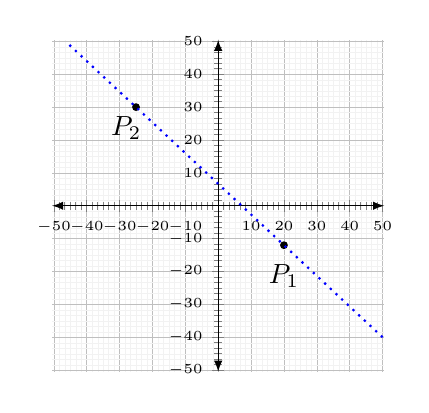
\begin{tikzpicture}
        \begin{axis}[
                width=\textwidth,
                scale=0.40,
                height=\textwidth,
                xtick distance=10,
                ytick distance=10,
                xmin=-50.0,xmax=50,
                ymin=-50.0,ymax=50,
                grid=both,
                grid style={line width=.1pt, draw=gray!10},
                major grid style={line width=.2pt,draw=gray!50},
                axis lines=middle,
                minor tick num=5,
                enlargelimits={abs=0.5},
                axis line style={latex-latex},
                ticklabel style={font=\tiny},
                xlabel style={at={(ticklabel* cs:1)},anchor=north west},
                ylabel style={at={(ticklabel* cs:1)},anchor=south west}
            ]
            
			\node at (-25,30) [circle,fill,inner sep=1pt]{};
		    \draw node[below] at (-28, 30) {$P_2$};
		    
		    \node at (20,-12) [circle,fill,inner sep=1pt]{};
		    \draw node[below] at (20, -15) {$P_1$};
		    
		    \draw[blue, thick, dotted] (50,-40) --  (-46.429,50);
            
    		\end{axis}
	\end{tikzpicture}
	\vspace{2em}
\end{center}

Above, we have a graph of 2 points: $P_1$ and $P_2$. Given these two points, the pointsBetween function aims to return a list of $n$ number of points that are a distance $w$ apart from each other and that lay on the line formed by $P_1$ and $P_2$(as shown in blue). To do this, we'll define a few variables: Let $d =$ the distance between $P_1$ and $P_2$, $n =$ the distance between each point(given), and $w =$ the scale factor. Specifically, $w$ will tell us how to modify our vector, but we'll get back to this in a second.


\begin{equation}
\begin{aligned}
	d &= \sqrt[2]{(x_{P1} - x_{P2})^2 + (y_{P1} - y_{P2})^2} \\
	w &= \frac{d}{n} \\
	n &= 2
\end{aligned}
\end{equation}

\vspace{1em}

Above, we use the pythagorean theorem to calculate $d$ which, once again, tells us the length of $\overline{\rm P_1P_2}$. Then, we calculate $w$ by dividing $d$ by $n$. Why? Well, when we divide $d$(the distance between the $P_1$ and $P_2$) by $n$(the distance we want between 2 points on $\overleftrightarrow{P_1P_2}$), we get a value which is equivalent to the number of points that we can generate between $P_1$ and $P_2$ when each point is a distance of $n$ away from its neighboring point. With this in mind, let's move on to the vector portion of this problem.

\end{document}